%\section{Runtime Architecture}

\subsection{Runtime}
\label{sec:runtime}

\begin{figure}
		\centering
		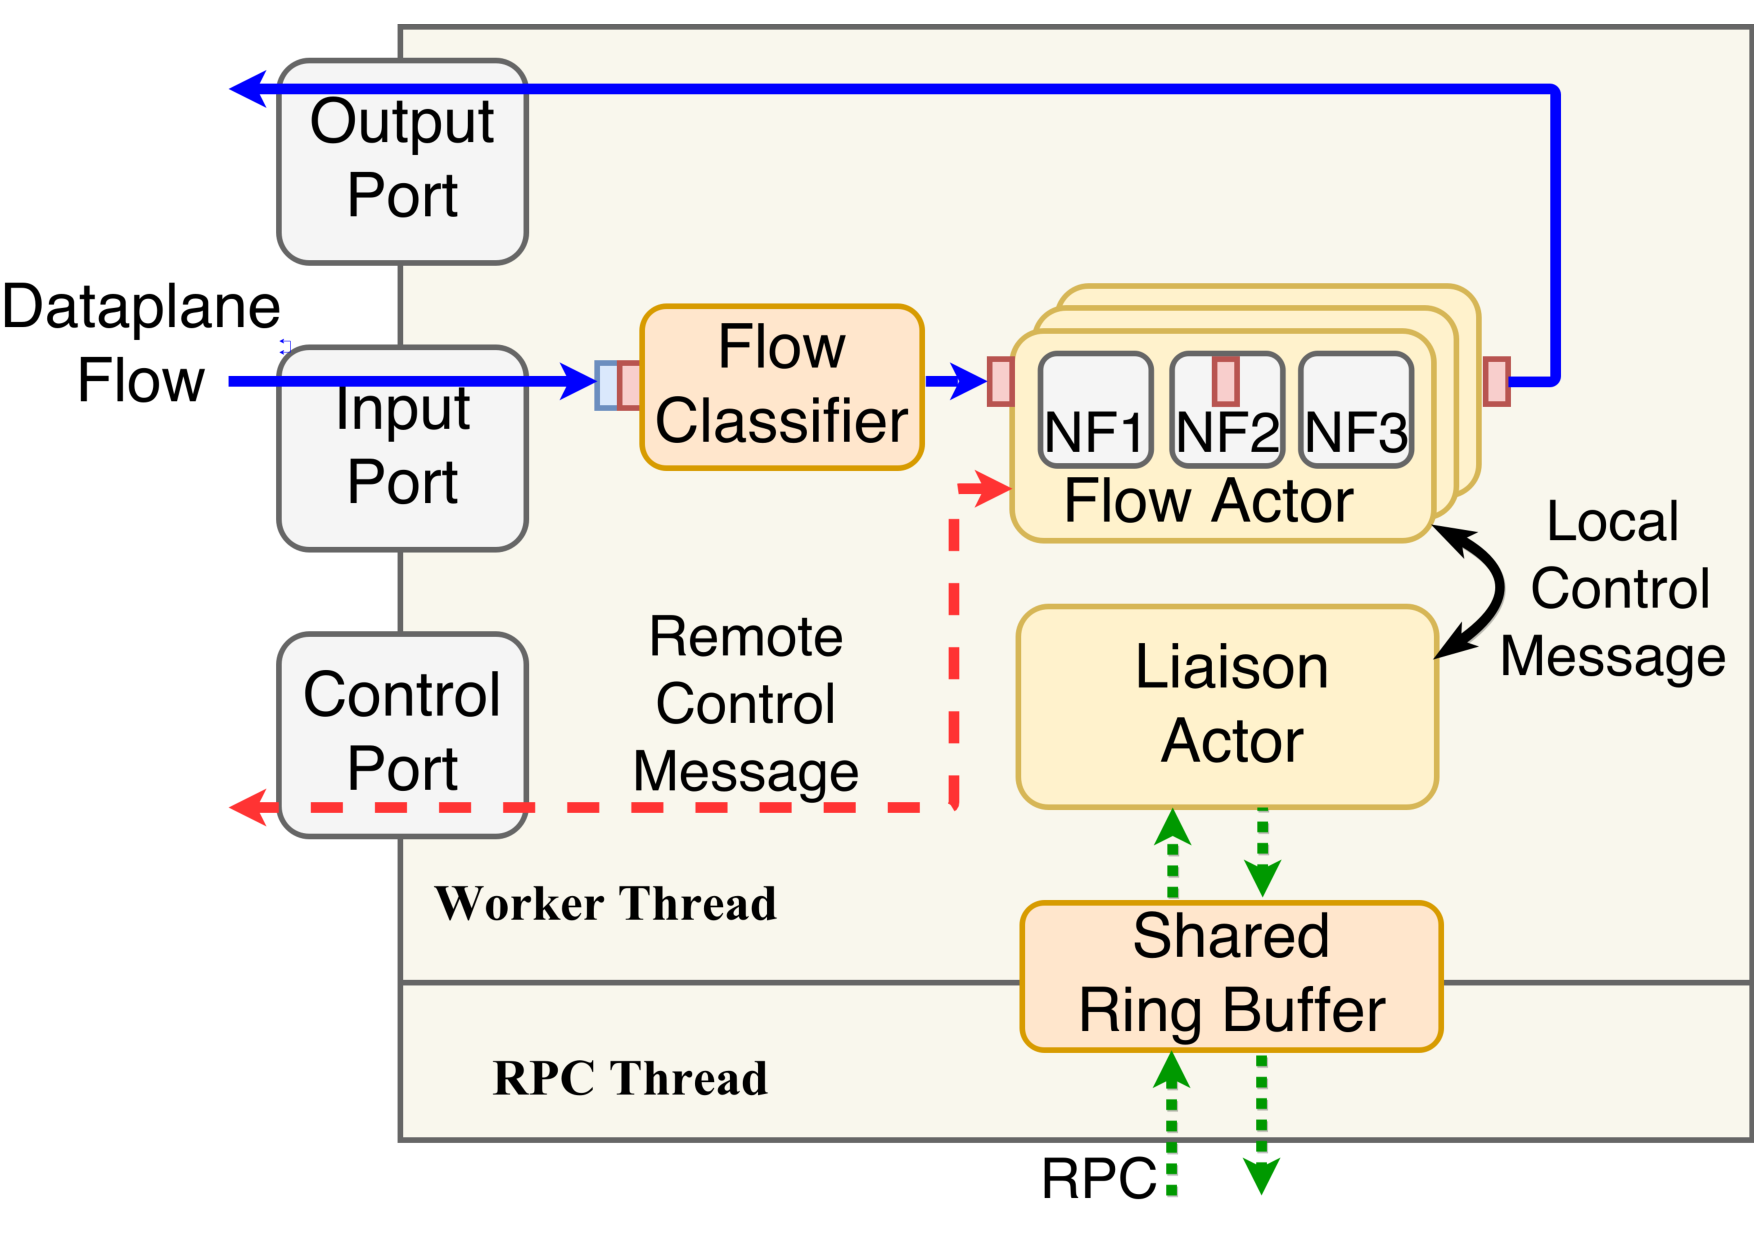
\includegraphics[width=\columnwidth]{figure/new-nfactor-runtime-arch.pdf}

		\caption{The internal structure of a runtime in \nfactor.}
\label{fig:runtime-arch}
\end{figure}

The concept of a uniform runtime system, as a basic flow processing and scaling unit in \nfactor, does not appear in most existing work \cite{bremler2015openbox, gember2012stratos, palkar2015e2}. In existing NFV systems, the basic flow processing and scaling unit is an NF instance, which is a virtual machine or container hosting an instance of a NF. % and the NF instances are chained on the data-plane. % The flows must go through these NF instances in sequence. 
 The primary reason that we design such a runtime is to enable NFs/service chains to achieve failure resilience automatically without coordinator intervention, as the runtime provides a network transparent abstraction \chuan{change this `network transparent' to a more accurate wording} to communicate and exchange messages among each other, which are crucial for flow migration and replication. 
  Especially, in a runtime, we adopt the simple yet powerful design to create a micro execution context for each flow, and encapsulate processing functions of the flow over its entire service chain inside the micro execution context. Then we can enable failure resilience on the basis of each micro execution context (Sec.~\ref{sec:resilience}). To be able to process multiple flows, the runtime is capable of handling multiple micro execution contexts concurrently. 

In \nfactor, we exploit the actor programming model to implement the micro execution context. Each micro execution context is a flow actor. Flow processing by NFs in the service chain, flow migration and replication functionalities are all implemented as message handlers of the flow actor. The runtime provides the basic runtime environment for all the flow actors that it has created. 


Fig.~\ref{fig:runtime-arch} shows the internal structure of a runtime. The input and output ports are used for receiving and sending flow packets from and to virtual switches. The control port is used for transmitting and receiving control messages exchanged among different runtimes for flow migration and replication, which are directly encapsulated inside L3 packets and sent/received using DPDK. %Both input port and output port could be used transmit and send actor messages as well, for instance, during the second request-response in the flow migration and during flow recovery.
 Input packets of dataplane flows are first sent to a flow classifier, which uses the classical 5-tuple of a flow (\ie, source IP address, destination IP address, transport-layer protocol, source port and destination port) to identify packets belonging to the same flow. One flow actor is created for each new flow. The flow actor loads NFs of the service chain configured in the runtime. All packets of the same flow are sent to the same flow actor, which processes them in sequence by passing them through NFs in the service chain. 
 
Each runtime is configured with a specific service chain by the coordinator during its booting phase. The runtime installs and initializes all the NFs as specified in the service chain upon booting. When a flow actor is created, it loads these NFs and uses a number of carefully defined NF APIs, as given in Table \ref{table:api} in Sec.~\ref{sec:NFAPIs}, to allocate flow states \chuan{not clear what `allocate flow states' means. extract?} and xxx \chuan{describe what it does to facilitate flow migration and replication by rewriting the idea of the following sentence: `Besides service chain processing, the flow actor also provides an execution context for distributed flow migration and replication, in response to certain messages (Sec.~\ref{sec:resilience})'}. 


Each runtime can host one or multiple flow actors for flows passing through the same service chain that the runtime is configured with, depending on its resource availability and performance isolation requirements. In case of a multi-tenant NFV system, we can run actors processing flows of the same tenant on the same runtime, but those of different tenants on different runtimes, for better security and isolation. When multiple flow actors are concurrently running on one runtime, they are scheduled by a worker thread: \chuan{clearly describe how the flow actors are scheduled} whenever a message is received at the actor's mailbox, .... In addition, our design of the NF modules in the next section will show that passing packets to a NF for processing in a flow actor is essentially just a function call; only one copy of each NF software needs to be loaded in a runtime, while the flow actors can all make use of it. %An actor itself is a very lightweight one as millions of actors could be spawned in seconds \cite{chs-rapc-16}. 



The runtime also consists of a RPC thread for receiving RPC requests from the coordinator (for flow migration, replication, etc.) and responding to them. The RPC thread and the worker thread share a ring buffer, used for relaying RPC requests received by the RPC thread to a liaison actor in the worker thread. We use a high-speed shared ring buffer to achieve fast inter-thread communication \chuan{add citation}. The liaison actor is responsible for coordinating with flow actors to execute the RPC requests from the coordinator. % flow actor initialization, flow migration and flow replication. %Flow actor and coordinator actor could directly exchanges local messages, or exchange remote messages through a reliable message passing module \cite{}.





\vspace{1mm}
\noindent {\bf Discussions on Runtime Design Choices.} The design of supporting only one service chain in one runtime significantly reduces the overhead of installing many NFs and avoids service chain selection in one runtime, for higher packet processing efficiency (speed) and management simplicity. Our one-actor-one-flow design is useful for facilitating fast flow migration (Sec.~\ref{sec:resilience}), which migrates a flow by migrating the actor that processes it \chuan{revise to more accurate description}. There are a few possible alternatives to our one-actor-one-flow design: (1) {\em One flow actor handles multiple flows.} It compromises the efficiency of flow migration, especially when multiple flows come from different virtual switch actors. In this case, the flow actor must synchronize the responses sent from different virtual switch actors \chuan{clarify what are `responses sent from different virtual switch actors' and why the flow actor needs to sync them}, adding overhead to flow migration process. (2) {\em One flow actor runs one NF}. Additional overhead is needed for chaining multiple flow actors to constitute a service chain, lowering packet processing speed. %Therefore, the one-flow-one-actor design achieves a sweet point in minimizing the actor processing overhead and improving the efficiency of flow migration protocol design.
Instead of using multiple worker threads in a runtime, the single-worker-thread design guarantees a sequential execution order of flow actors, thereby completely eliminating the need to protect message passing by locks \chuan{message passing among flow actors or what?}, and achieving higher efficiency. 




%The alternative design to one-runtime-one-service-chain is to dynamically configure multiple service chains on a single runtime. Then due to the one-flow-one-actor design, we need to do an additional service chain selection, based on some pre-defined rules. This adds additional overhead to the flow actor processing and increases the complexity when managing the NFActor cluster, because the controller must populates the service chain rule dynamically to each runtime. With the one-runtime-on-service-chain design, if another service chain is needed, the system administrator could launch a new NFActor cluster and configure a different service chain to use.




%The runtime is designed as a single-worker-thread architecture to decrease the overhead of flow actors. A high speed NFV system may process millions of packets every second and migrates tens of thousands of flows. At such a high processing rate, message passing protected by shared lock in multi-threaded actor runtime system may incur a huge overhead and hurt the packet throughput.
%The runtime is configured with a specific service chain during the boot phase and initializes all the NF modules as specified in the service chain. When a flow actor is created, it loads these modules and uses the flow state allocation method \ref{table:api} to allocates all the
%To process flows across a service chain, during the initialization phase of the runtime, a service chain specifier is passed in to the runtime. The runtime then loads all the NF modules as indicated in the service chain specifier. When the flow classifier creates a new flow actor, the flow actor also loads these NF modules on the service chain and passes the input packet along the NF modules in sequence.

%The reason that the runtime is designed as a single-worker-thread program is because the multi-worker-thread design may not bring significant performance gain. In our initial prototype implementation, we use LIBCAF \cite{caf} library to construct flow actors. LIBCAF library creates multiple worker threads and schedules flow actors to run on these worker threads. Because LIBCAF completely conceals the internal interfaces of the worker threads, we have to create a dedicated polling thread to poll packet from the input port. Under this design, we find that the maximum throughput of a runtime does not increase when the number of LIBCAF worker thread increases, because the polling thread has always been a bottleneck. Therefore, we abandon the multi-worker-thread design and use a single worker thread to poll packets and schedule flow actors. To our surprise, this architecture turns out to work very well because it allows us to perform aggressive optimization of actor programming model \ref{}. In the mean time, we can still maintain the scalability of the system by launching more runtimes.

\subsection{NF APIs}
\label{sec:NFAPIs}

To achieve transparent resilience together with the micro execution environments provided by runtimes in \nfactor, an important step is to separate useful NF states from the core processing logic of each NF. With this separation, a flow actor can retrieve and serialize NF states for transmission whenever needed, without interfering with packet processing of the NF. In \nfactor, we achieve this separation by designing a set of APIs that NF implementation should follow in \nfactor. 
 
\begin{table}[!t]
\centering
\caption{APIs to be Implemented by NFs in \nfactor.}
\label{table:api}
\resizebox{\columnwidth}{!}{
\begin{tabular}{c|l}
\textbf{API}                                      & \multicolumn{1}{c}{\textbf{Usage}}                                                                                                                                                                                                         \\ \hline
nf.allocate\_new\_fs()                            & \begin{tabular}[c]{@{}l@{}}Create a new flow state object for\\ a new flow actor, to be used for storing flow state\end{tabular}                                                                                                                                                  \\ \hline
nf.deallocate\_fs(fs)                             & \begin{tabular}[c]{@{}l@{}}Deallocate the flow state object\\ when the flow actor expires\\\end{tabular}                                                                                                                               \\ \hline
nf.process\_pkt(input\_pkt, fs)                   & \begin{tabular}[c]{@{}l@{}}Process the input packet using the \\ current flow state\end{tabular}                                                                                                         \\ \hline
%nf.get\_migration\_target(cluster\_cfg, fs) & \begin{tabular}[c]{@{}l@{}}Query an NF using the current\\ cluster configuration and \\ flow state about which runtime this flow\\ actor should be migrated to\end{tabular} \\ \hline
\end{tabular}
}
\end{table}


The APIs are given in Table \ref{table:api}, provided as four public methods for each NF to implement. When a new flow actor is created to handle a new flow, it first calls $nf.allocate\_new\_fs()$ to create a flow state object. Whenever the actor receives a new packet, the actor passes the received packet and the flow state object to \\
$nf.process\_pkt(input\_pkt, fs)$, for processing by the NFs, in sequence of the service chain. Any changes to the flow state when an NF has processed the packet is immediately visible to the flow actor. When the flow terminates, the flow actor expires and it calls $nf.deallocate\_fs(fs)$ to deallocate the flow state object. Using these three APIs, the flow actor always has direct access to the latest flow state, enabling it to transmit the flow state during flow migration and replication processes without disturbing packet processing of the NFs. %Therefore, the combination of the three methods servers as the basis for the transparent resilience in~\nfactor. 

%\chuan{add the idea to flow migration section rather than exposign the API here} The fourth API $nf.get\_migration\_target(cluster\_cfg, fs)$ is used for checking where the NF would like the actor to migrate to, by passing the current cluster configuration and the current flow state. This enables the flow actor to actively migrate itself instead of waiting for migration initiation command sends from the controller \ref{}. This distributed design is the key to sparkle several useful applications, \ie, flow deduplication and reliable MPTCP subflow processing, which we will discuss in Sec.~\ref{sec:experiments}, that existing NFV systems based on centralized flow management cannot achieve. The flow actor should only call this method on the last NF in the service chain. Therefore NFs modules implementing this method should be placed on as the last NF in the service chain. 

%These three methods are simple to use and properly generalize the structure of NFs that processes flow packets based on per-flow state. Using these three methods, we are able to create several representing NFs as shown in \ref{}.}

%The flow actor acquires the flow state of all the NF modules using the allocation API, and passes the packet across all the NF modules in sequence using the processing API.


To implement an NF in \nfactor, core processing logic of the NF needs to be implemented following the actor model and the APIs in Table \ref{table:api}. Nevertheless, porting the core
processing logic of an existing NF software is relatively straightforward. We have implemented a broad range of NFs in \nfactor and will present details in Sec.~\ref{sec:experiments}.


\subsection{Virtual Switch}
\label{sec:virtualswitch}

A virtual switch in \nfactor~is a special runtime where the actors do not run a service chain but only a load balancer function. Following the one-actor-one-flow principle, a virtual switch can create multiple actors each to dispatch packets belonging to one flow. We refer to a flow dispatching actor in a virtual switch as a {\em virtual switch actor}. 


Each virtual switch receives information of the runtimes that it can dispatch flows to from the coordinator, through RPC requests its liaison actor receives, including MAC addresses of the input ports of the runtimes. A virtual switch actor selects one of the runtimes to forward its flow in a round-robin fashion, upon creation of this actor. We choose a simple round-robin approach because the virtual switch must run very fast and a round-robin algorithm introduces the smallest amount of overhead while providing satisfactory load balancing performance. Whenever a virtual switch actor receives an incoming packet, it replaces the destination MAC address of the packet to MAC address of input port of the chosen runtime, modifies the source MAC address of the packet to MAC address of output port of the virtual switch, and then sends the packet out from the output port.

The architectural consistency of virtual switches and runtimes in \nfactor~facilitates flow migration and replication. The flow actor on a runtime can analyze the source MAC address of the incoming packets and determine which virtual switch this packet comes from. Then the flow actor can contact the virtual switch during flow migration and replication processes, to indicate change of the runtime that the respective virtual switch actor should dispatch packets to. This is done through remote control message exchanges with the virtual switch in the same way as message exchanges with other runtimes.

\chuan{describe how the virtual switches are used for receiving outgoing packets from runtime and send them to final destinations}

Existing NFV management systems either rely on SDN switches \cite{gember2012stratos, gember2015opennf} to route flows from one NF to the next, or build a customized data-plane for inter-connecting different NF instances \cite{palkar2015e2}. In comparison, our virtual switch is lightweight, only to dispatch flows to runtimes, but not route flows through individual NFs.


\subsection{Coordinator}
\label{sec:coordinator}

The \nfactor's coordinator is responsible for launching new virtual switches and runtimes, monitoring the load on each runtime and executing dynamic scaling. Due to our distributed flow actor design, the coordinator only needs to participate in the initiation phase of flow migration and replication (Sec.~\ref{sec:resilience}). This differentiates \nfactor's coordinator with the controllers in existing NFV systems \cite{gember2015opennf}\cite{rajagopalan2013split}, which need to fully coordinate the entire flow migration process. 
The design of the coordinator is simplified and improve failure resilience of the system is improved, as the coordinator does not need to maintain complicated states associated with flow migration.

To deploy a service chain in \nfactor, the system administrator first specifies composition of the service chain to the coordinator, as well as several rules to match the input flows to service chains. \chuan{describe how you use SDN or openflow like rules to enable dispatching flows to correct virtual switches}. The coordinator then launches a new virtual switch and a new runtime, configures the runtime with this service chain, and directs incoming flows using the service chain to the virtual switch. Each runtime or virtual switch is assigned a global unique ID to ease management.  In \nfactor, a virtual switch is responsible for dispatching flows using the same service chain, to runtimes installed with this service chain. The virtual switches and runtimes handling the same service chain are referred to as a {\em cluster} in \nfactor. Flow migration and replication occur within a cluster. These design choices are made since xxx \chuan{give the rationale}.


Each runtime in \nfactor~regularly sends heartbeat messages to the coordinator, containing the current load information (\ie, CPU usage, memory usage) of the runtime. When the coordinator detects that a runtime is overloaded, it scales up the cluster by launching a new runtime and configures the service chain on that runtime (Sec.~\ref{}\chuan{point to the scaling section}). \chuan{does the coordinator takes care of virtual switch scaling as well? describe it}

The coordinator communicates with runtimes via a series of control RPCs exposed by each runtime, as summarized in Table \ref{table:rpc}. It uses $PollWorkload()$ to acquire the current load on a runtime, to produce scaling decision. The coordinator maintains the composition of the system, which includes the mac addresses of input/output/control ports and the IDs of all runtimes and virtual switches of all clusters (handling different service chains). The coordinator updates a runtime composition of the runtime it belongs to using $NotifyClusterCfg(cfg)$ \chuan{does coordinator sends it to virtual switches as well?}. The cluster composition learned by different runtimes in a cluster do not have to be consistent because our flow migration and replication protocols perform safety checking by exchanging requests and responses to eliminate the inconsistency \chuan{check if this is true and revise accordingly}. The last three RPCs are used to initiate flow migration and replication. After issuing these three calls, migration and replication are automatically executed without further involving the coordinator.
\chuan{briefly describe why you use RPC for coordinator to runtime communication.}



\begin{table}[!t]
\centering
\caption{Control RPCs Exposed at Each Runtime}
\label{table:rpc}
\resizebox{\columnwidth}{!}{
\begin{tabular}{l|l}
Control RPC                                                                                   & Functionality                                                                                                                                              \\ \hline
PollWorkload()                                                                                   & \begin{tabular}[c]{@{}l@{}}Poll the load information \\ from a runtime.\end{tabular}                                                                 \\ \hline
NotifyClusterCfg(cfg)                                                                         & \begin{tabular}[c]{@{}l@{}}Notify a runtime the current \\ cluster view.\end{tabular}                                                             \\ \hline
\begin{tabular}[c]{@{}l@{}}SetMigrationTarget(runtime\_id, \\ migration\_number)\end{tabular} & \begin{tabular}[c]{@{}l@{}}Initiate flow migration. It tells \\ the runtime to migrate \\ migration\_num of flows to the runtime\\ with runtime\_id.\end{tabular} \\ \hline
SetReplica(runtime\_id)                                                                       & \begin{tabular}[c]{@{}l@{}}Set the runtime with runtime\_id \\ as the replica.\end{tabular}                                                                \\ \hline
Recover(runtime\_id)                                                                          & \begin{tabular}[c]{@{}l@{}}Recover all the flows replicated \\ from runtime with runtime\_id.\end{tabular}                                                 \\ \hline
\end{tabular}
}
\end{table}